\section{Numerical Results}
In this section the simulation results are presented. The simulated system is a pure double integrator with two states and two inputs. The model reference is chosen to be 



\begin{figure}[!t]
    \centering
    \begin{subfigure}[b]{0.49\linewidth}
     \centering
     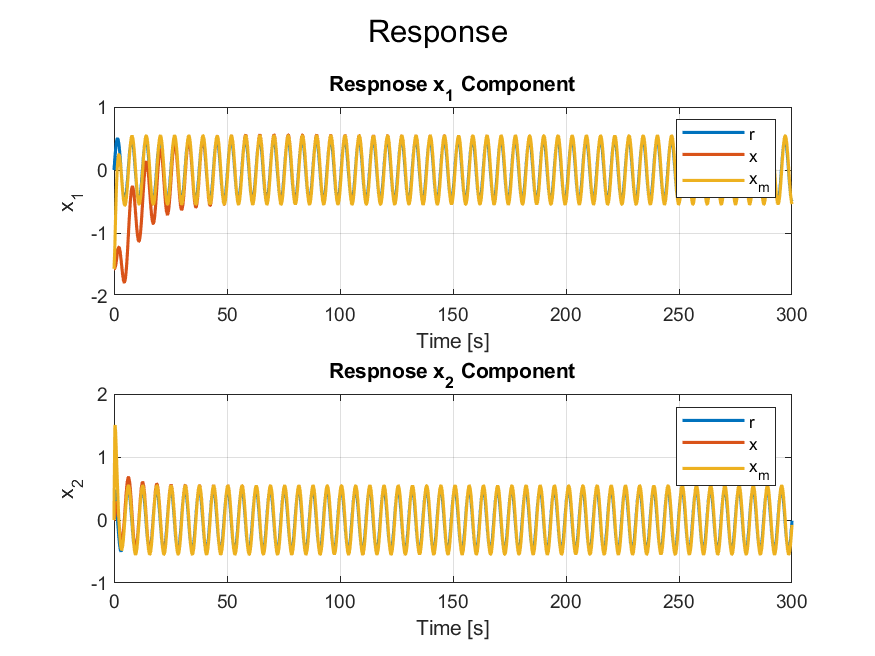
\includegraphics[width=\linewidth]{images/sine/NMRAC_MIMO_Response.png}
     \caption{Time response of simulated system}
     \label{fig:resonse-in-states}
    \end{subfigure}
    \hfill
    \begin{subfigure}[b]{0.49\linewidth}
     \centering
     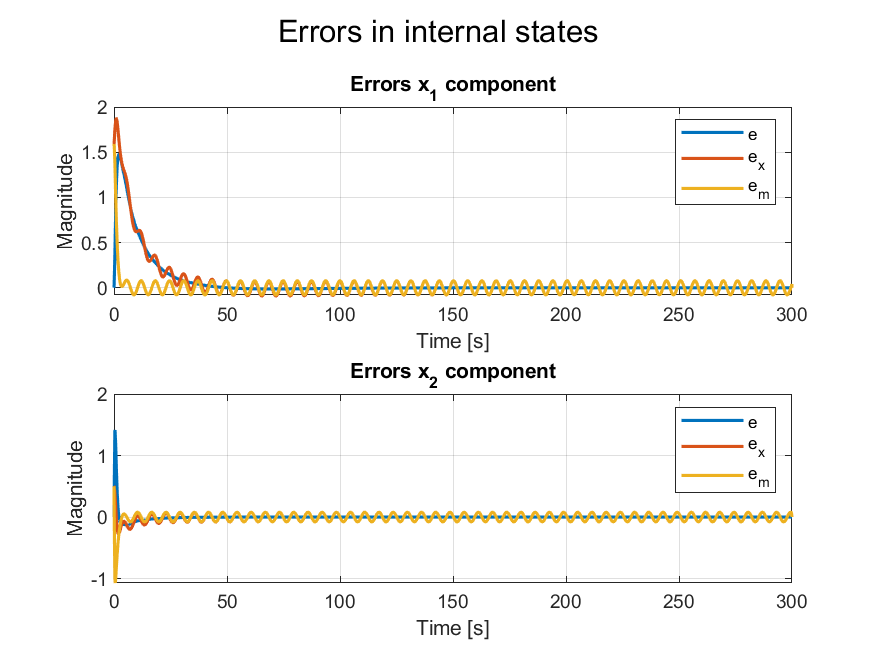
\includegraphics[width=\linewidth]{images/sine/NMRAC_MIMO_Error.png}
     \caption{Error in internal states}
     \label{fig:error}
    \end{subfigure}
    \caption{Lyapunov function and convergence of the system w.r.t. internal states and dynamics}
    \label{fig:response}
\end{figure}

\begin{figure}
    \centering
    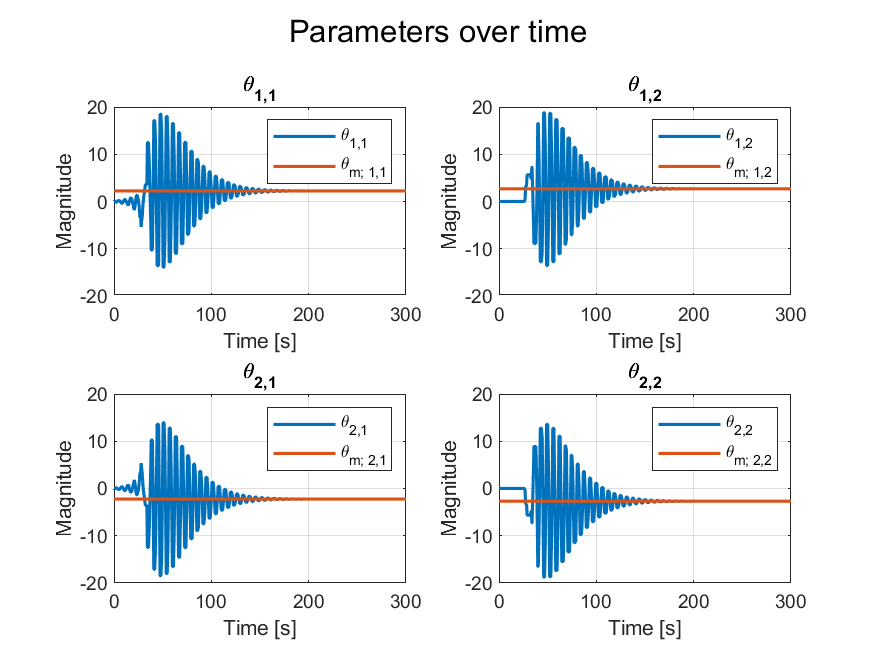
\includegraphics[width=\linewidth]{images/sine/NMRAC_MIMO_Parameters.png}
    \caption{Evolution of parameters over time}
    \label{fig:parameters}
\end{figure}


\begin{figure}[!t]
    \centering
    \begin{subfigure}[b]{0.49\linewidth}
     \centering
     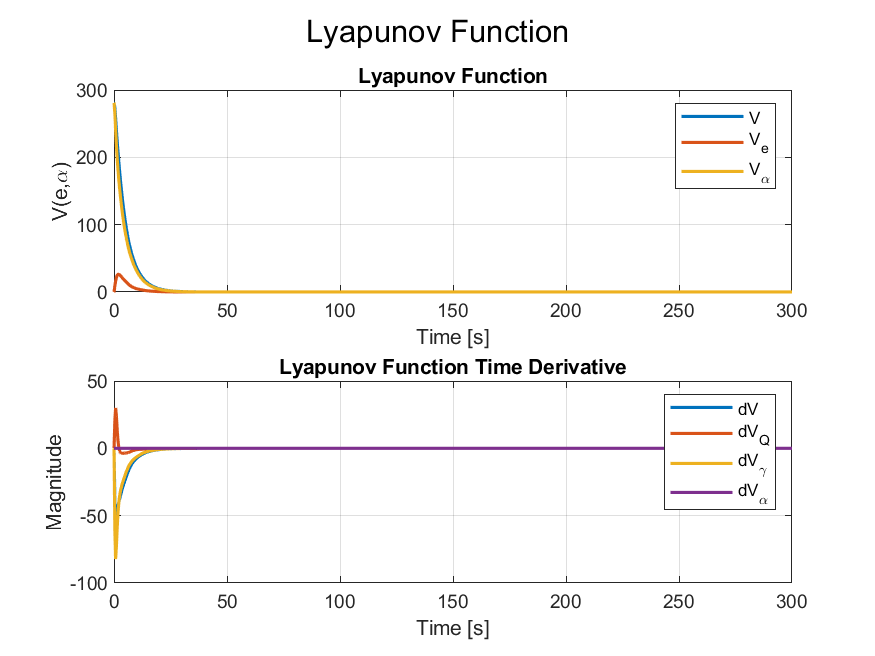
\includegraphics[width=\linewidth]{images/sine/NMRAC_MIMO_Lyapunov.png}
     \caption{Lyapunov function}
     \label{fig:Lyapunov-step-input}
    \end{subfigure}
    \hfill
    \begin{subfigure}[b]{0.49\linewidth}
     \centering
     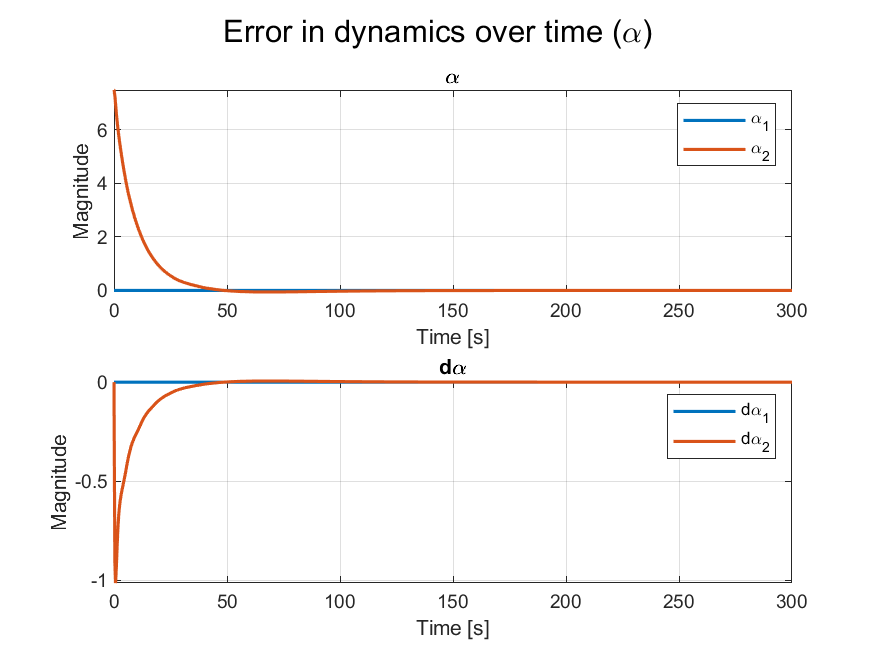
\includegraphics[width=\linewidth]{images/sine/NMRAC_MIMO_Alpha.png}
     \caption{Time derivative of the Lyapunov function}
     \label{fig:step-error}
    \end{subfigure}
    \caption{Lyapunov function}
    \label{fig:step-lyap}
\end{figure}

\section{Implementation on a System}
